\documentclass[border=10pt]{standalone}
\usepackage{tikz}
\definecolor{myred}{RGB}{190,60,45}
\definecolor{myblue}{RGB}{38,84,160}
\begin{document}
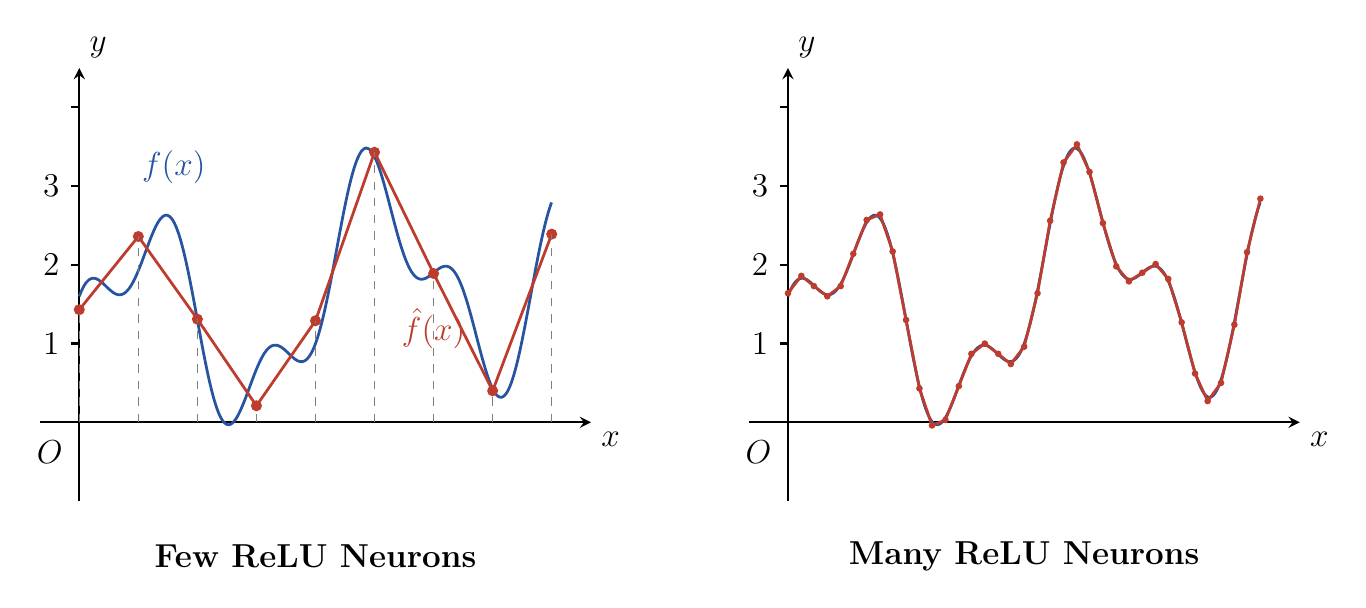
\begin{tikzpicture}[>=stealth, line width=0.8pt, font=\large,
    declare function={f(\x) = 1.2*sin(\x*120) + 0.6*cos(\x*300) + 0.2*\x + 1;}]

  % ===== 左：8 段真最小二乘拟合（欠拟合）=====
  \begin{scope}[xshift=0cm]
    \draw[->] (-0.5,0) -- (6.5,0)   node[below right] {$x$};
    \draw[->] (0,-1.0) -- (0,4.5)   node[above right] {$y$};
    \coordinate (origin) at (0,0);
    \foreach \t in {1,2,3,4} \draw (0,\t) -- ++(-0.1,0);
    \foreach \t in {1,2,3}   \node[left] at (-0.12,\t) {$\t$};
    \node[below left] at (-0.08,-0.1) {$O$};
    \draw[myblue, line width=1pt, smooth, samples=200, domain=0:6]
      plot (\x, {f(\x)});
    \node[myblue] at (1.2,{f(1.2)+0.7}) {$f(x)$};
    \draw[myred, line width=1pt] plot coordinates {(0.00,1.43) (0.75,2.36) (1.50,1.31) (2.25,0.21) (3.00,1.29) (3.75,3.43) (4.50,1.89) (5.25,0.40) (6.00,2.39)};
    \node[myred] at (4.5,1.19) {$\hat{f}(x)$};
    \fill[myred] (0.00,1.43) circle (2pt); \draw[gray, dashed, line width=0.5pt] (0.00,0) -- (0.00,1.43);
    \fill[myred] (0.75,2.36) circle (2pt); \draw[gray, dashed, line width=0.5pt] (0.75,0) -- (0.75,2.36);
    \fill[myred] (1.50,1.31) circle (2pt); \draw[gray, dashed, line width=0.5pt] (1.50,0) -- (1.50,1.31);
    \fill[myred] (2.25,0.21) circle (2pt); \draw[gray, dashed, line width=0.5pt] (2.25,0) -- (2.25,0.21);
    \fill[myred] (3.00,1.29) circle (2pt); \draw[gray, dashed, line width=0.5pt] (3.00,0) -- (3.00,1.29);
    \fill[myred] (3.75,3.43) circle (2pt); \draw[gray, dashed, line width=0.5pt] (3.75,0) -- (3.75,3.43);
    \fill[myred] (4.50,1.89) circle (2pt); \draw[gray, dashed, line width=0.5pt] (4.50,0) -- (4.50,1.89);
    \fill[myred] (5.25,0.40) circle (2pt); \draw[gray, dashed, line width=0.5pt] (5.25,0) -- (5.25,0.40);
    \fill[myred] (6.00,2.39) circle (2pt); \draw[gray, dashed, line width=0.5pt] (6.00,0) -- (6.00,2.39);
    \node[font=\large\bfseries] at (3,-1.7) {Few ReLU Neurons};
  \end{scope}

  % ===== 右：36 段真最小二乘拟合（万能逼近）=====
  \begin{scope}[xshift=9cm]
    \draw[->] (-0.5,0) -- (6.5,0)   node[below right] {$x$};
    \draw[->] (0,-1.0) -- (0,4.5)   node[above right] {$y$};
    \coordinate (origin) at (0,0);
    \foreach \t in {1,2,3,4} \draw (0,\t) -- ++(-0.1,0);
    \foreach \t in {1,2,3}   \node[left] at (-0.12,\t) {$\t$};
    \node[below left] at (-0.08,-0.1) {$O$};
    \draw[myblue, line width=1pt, smooth, samples=200, domain=0:6]
      plot (\x, {f(\x)});
    \draw[myred, line width=1pt] plot coordinates {(0.00,1.64) (0.17,1.86) (0.33,1.73) (0.50,1.60) (0.67,1.73) (0.83,2.14) (1.00,2.57) (1.17,2.64) (1.33,2.17) (1.50,1.30) (1.67,0.43) (1.83,-0.04) (2.00,0.03) (2.17,0.46) (2.33,0.87) (2.50,1.00) (2.67,0.87) (2.83,0.74) (3.00,0.96) (3.17,1.64) (3.33,2.56) (3.50,3.30) (3.67,3.53) (3.83,3.18) (4.00,2.53) (4.17,1.98) (4.33,1.79) (4.50,1.90) (4.67,2.01) (4.83,1.82) (5.00,1.27) (5.17,0.62) (5.33,0.27) (5.50,0.50) (5.67,1.24) (5.83,2.16) (6.00,2.84)};
    \fill[myred] (0.00,1.64) circle (1.2pt);
    \fill[myred] (0.17,1.86) circle (1.2pt);
    \fill[myred] (0.33,1.73) circle (1.2pt);
    \fill[myred] (0.50,1.60) circle (1.2pt);
    \fill[myred] (0.67,1.73) circle (1.2pt);
    \fill[myred] (0.83,2.14) circle (1.2pt);
    \fill[myred] (1.00,2.57) circle (1.2pt);
    \fill[myred] (1.17,2.64) circle (1.2pt);
    \fill[myred] (1.33,2.17) circle (1.2pt);
    \fill[myred] (1.50,1.30) circle (1.2pt);
    \fill[myred] (1.67,0.43) circle (1.2pt);
    \fill[myred] (1.83,-0.04) circle (1.2pt);
    \fill[myred] (2.00,0.03) circle (1.2pt);
    \fill[myred] (2.17,0.46) circle (1.2pt);
    \fill[myred] (2.33,0.87) circle (1.2pt);
    \fill[myred] (2.50,1.00) circle (1.2pt);
    \fill[myred] (2.67,0.87) circle (1.2pt);
    \fill[myred] (2.83,0.74) circle (1.2pt);
    \fill[myred] (3.00,0.96) circle (1.2pt);
    \fill[myred] (3.17,1.64) circle (1.2pt);
    \fill[myred] (3.33,2.56) circle (1.2pt);
    \fill[myred] (3.50,3.30) circle (1.2pt);
    \fill[myred] (3.67,3.53) circle (1.2pt);
    \fill[myred] (3.83,3.18) circle (1.2pt);
    \fill[myred] (4.00,2.53) circle (1.2pt);
    \fill[myred] (4.17,1.98) circle (1.2pt);
    \fill[myred] (4.33,1.79) circle (1.2pt);
    \fill[myred] (4.50,1.90) circle (1.2pt);
    \fill[myred] (4.67,2.01) circle (1.2pt);
    \fill[myred] (4.83,1.82) circle (1.2pt);
    \fill[myred] (5.00,1.27) circle (1.2pt);
    \fill[myred] (5.17,0.62) circle (1.2pt);
    \fill[myred] (5.33,0.27) circle (1.2pt);
    \fill[myred] (5.50,0.50) circle (1.2pt);
    \fill[myred] (5.67,1.24) circle (1.2pt);
    \fill[myred] (5.83,2.16) circle (1.2pt);
    \fill[myred] (6.00,2.84) circle (1.2pt);
    \node[font=\large\bfseries] at (3,-1.7) {Many ReLU Neurons};
  \end{scope}

\end{tikzpicture}
\end{document}
